% Guia: flujos de usuario, wireframes y criterios de usabilidad y accesibilidad.
El nombre del sistema "Thary" fue elegido en la etapa de diseño de identidad visual, es un nombre corto escogido por fonéticamente sonar similar a las últimas cuatro letras de la palabra "Inventory", (inventario en inglés). En cuanto a icono representativo, se eligió la figura de un buho, para transmitir la idea de orden y control, ya que los buhos son animales reconocidos por su capacidad de percepción y vigilancia, relacionado a como Thary se encarga de detectar señales de riesgo que podrían afectar el inventario de una empresa.

\begin{figure}[H]
    \centering
    
\includegraphics[width=0.5\textwidth]{templatefigures/logo}
    \caption{Logotipo de Thary, compuesto por el nombre del sistema y el icono representativo del búho}
    \label{fig:ux_login_logo}
\end{figure}

Para realizar el diseño de interacción de Thary, se decidió separar las pantallas en dos: Una dirigida exclusivamente a los administradores y otra dirigida a los empleados del inventario. Al ingresar al sistema, un usuario con el rol de administrador sigue el siguiente flujo:

El usuario inicia sesión o se registra de no tener una cuenta.

\begin{figure}[H]
    \centering
    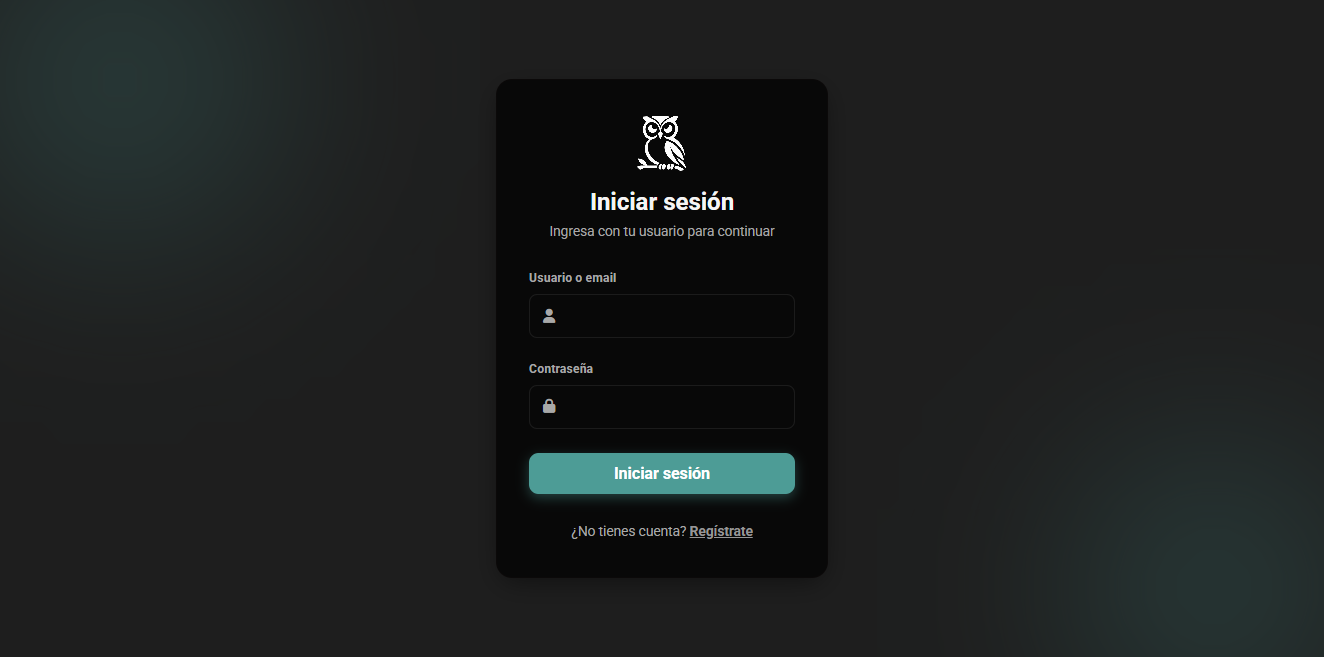
\includegraphics[width=0.5\textwidth]{templatefigures/ux_login}
    \caption{Pantalla de inicio de sesión de Thary}
    \label{fig:ux_login}
\end{figure}

\begin{figure}[H]
    \centering
    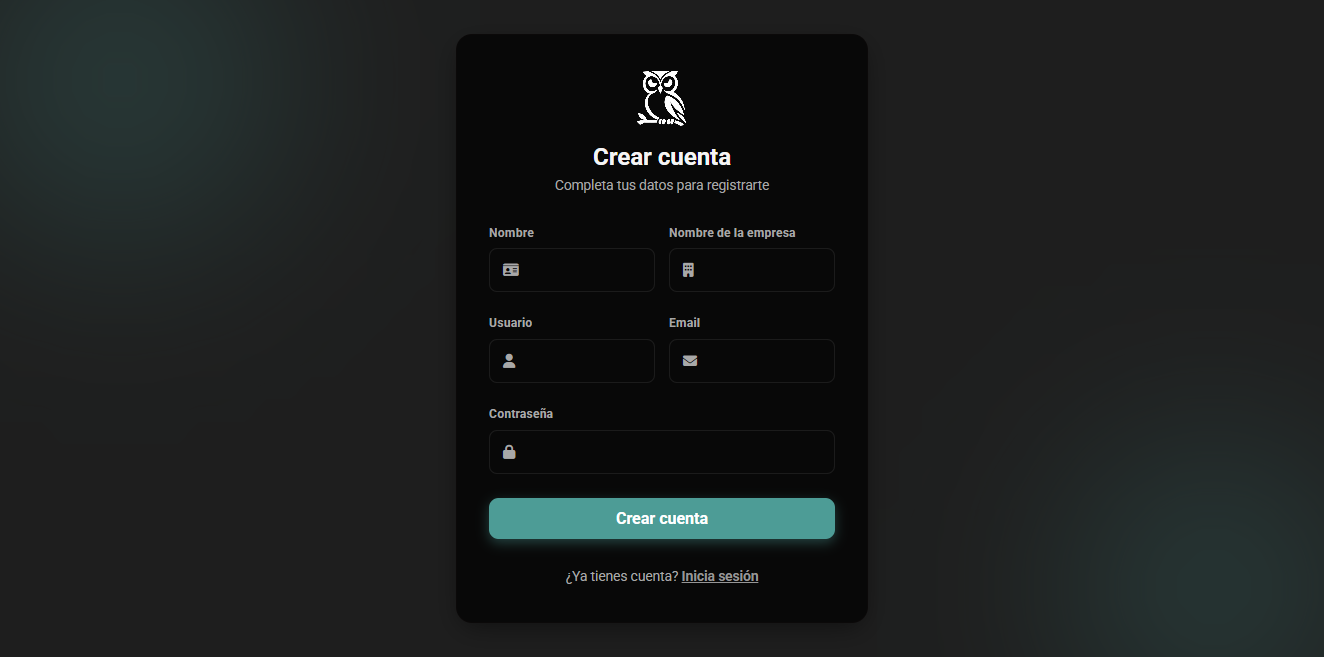
\includegraphics[width=0.5\textwidth]{templatefigures/ux_registro}
    \caption{Pantalla de registro de Thary}
    \label{fig:ux_registro}
\end{figure}

El administrador inicia en la pantalla de inicio del sistema, desde la cual puede acceder a la funcionalidad de carga de archivo (\textit{index}), al haber cargado el archivo correctamente y que este sea válido, se le redirige automáticamente al dashboard, donde al seleccionar "Pronóstico de demanda", se muestran los resultados.

\begin{figure}[H]
    \centering
    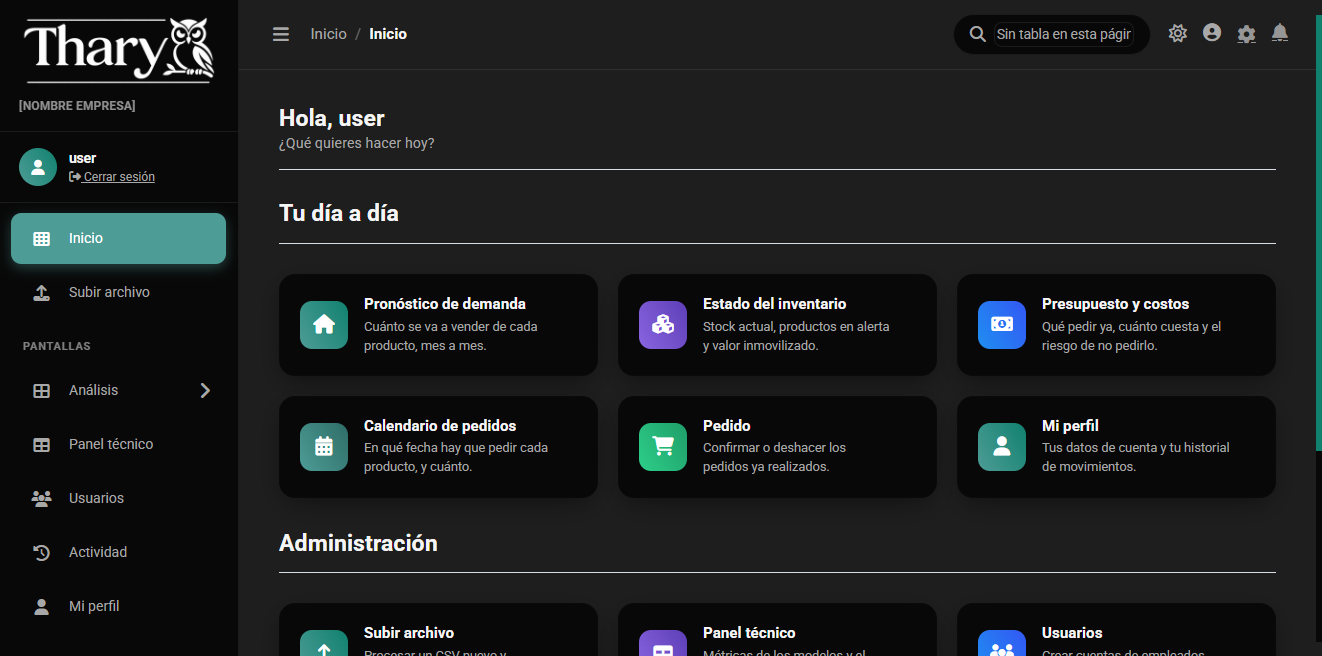
\includegraphics[width=0.5\textwidth]{templatefigures/ux_dashboard}
    \caption{Pantalla de dashboard de Thary}
    \label{fig:ux_dashboard}
\end{figure}


\begin{figure}[H]
    \centering
    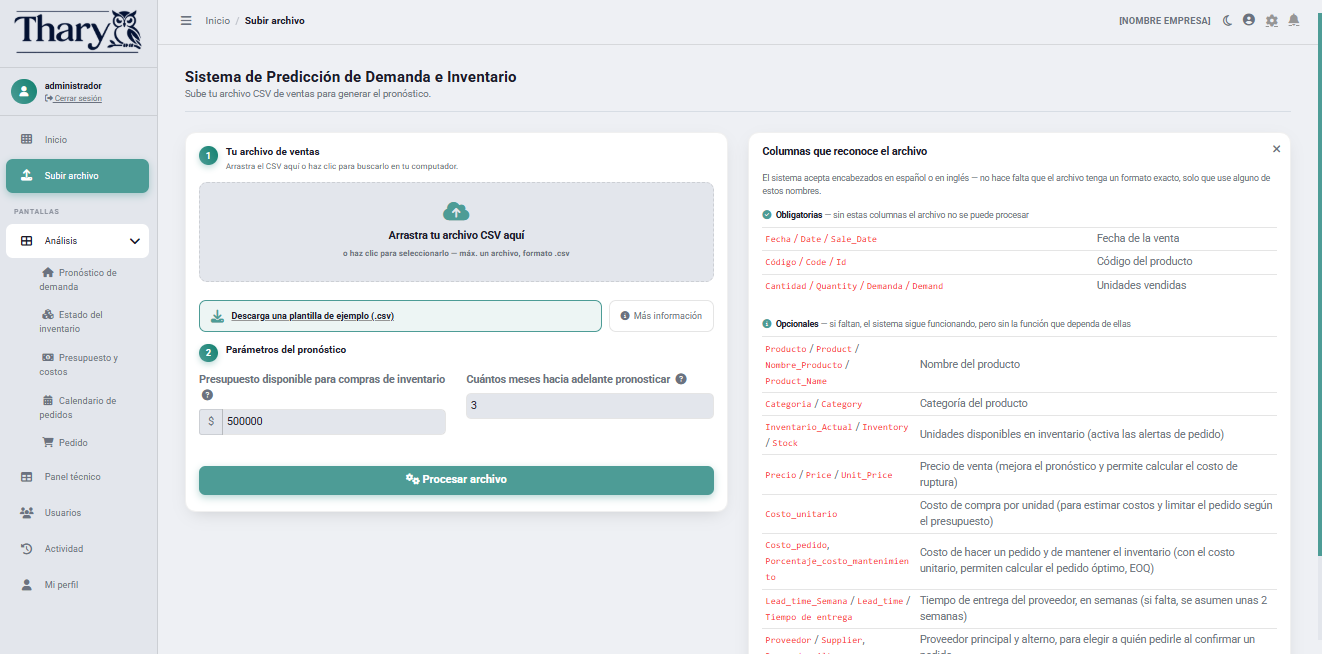
\includegraphics[width=0.5\textwidth]{templatefigures/ux_subir_archivo}
    \caption{Pantalla para subir archivos de Thary}
    \label{fig:ux_subir_archivo}
\end{figure}


\begin{figure}[H]
    \centering
    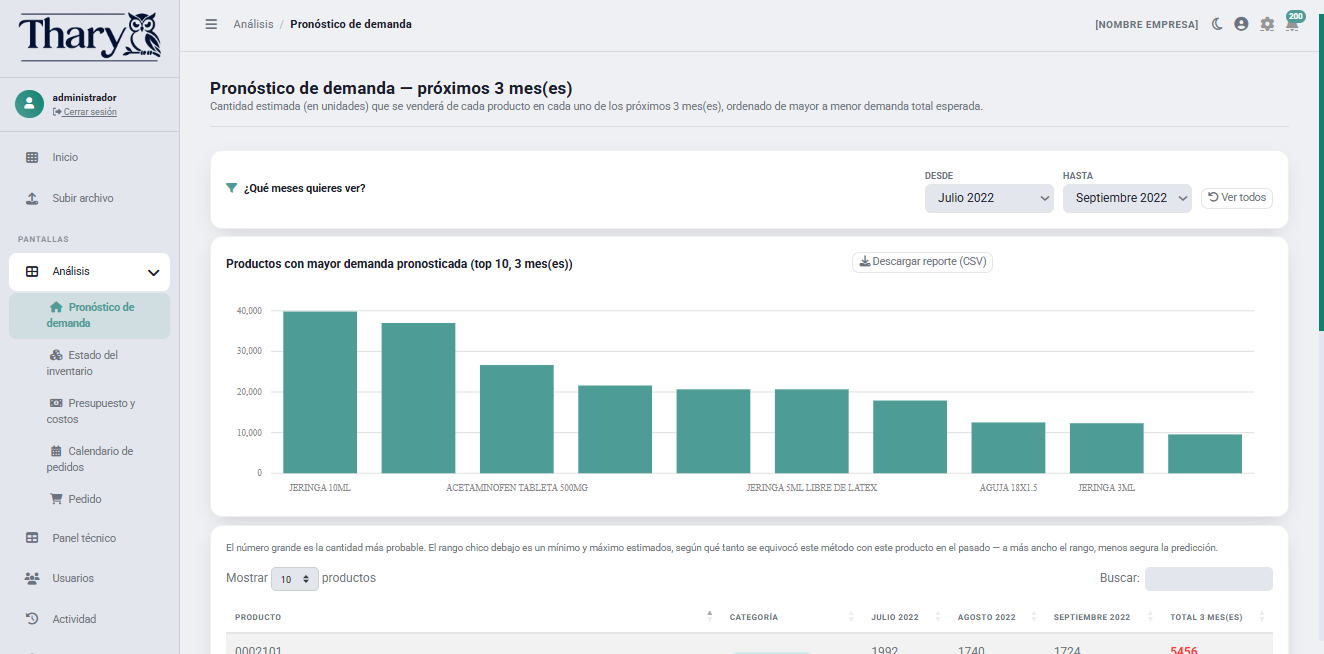
\includegraphics[width=0.5\textwidth]{templatefigures/ux_prediccion}
    \caption{Pantalla de predicción de demanda de Thary}
    \label{fig:ux_prediccion}
\end{figure}

En el sidebar, además de encontrar demas opciones como estado del inventario, presupuesto y pedidos, el administrador puede navegar hacia la gestión de usuarios, donde puede crear cuentas nuevas para su personal de inventario. 

\begin{figure}[H]
    \centering
    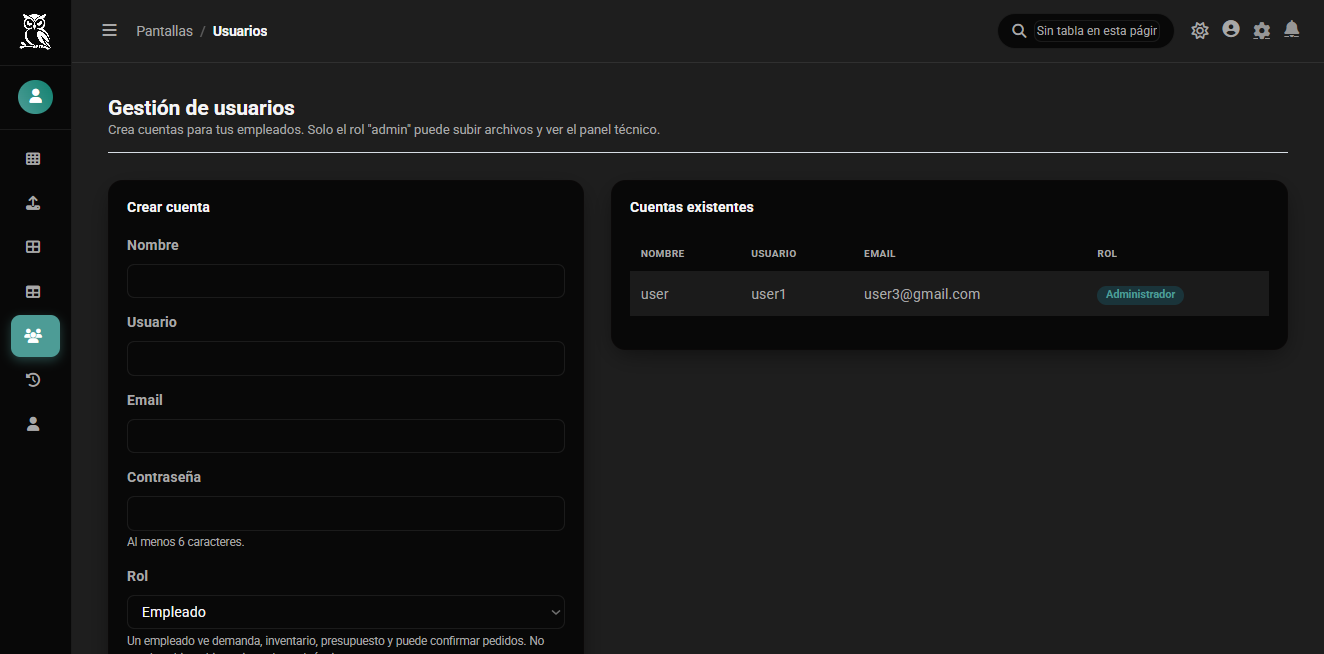
\includegraphics[width=0.5\textwidth]{templatefigures/ux_usuarios}
    \caption{Pantalla de gestión de usuarios de Thary}
    \label{fig:ux_usuarios}
\end{figure}

El flujo de los empleados es bastante similar, con la diferencia de que el perfil de un empleado cuenta con menos privilegios que el perfil de un administrador, por lo que al iniciar sesión, el empleado no puede subir ningún archivo,por lo que solo puede acceder al dashboard de la demanda pronosticada en base al csv que ya anteriormente fue cargado al sistema por el administrador que creó su cuenta, ya desde ahí, puede navegar a las mismas funcionalidades del análisis de los datos que el administrador: estado del inventario, presupuesto y pedidos. 

\begin{figure}[H]
    \centering
    \begin{subfigure}[b]{0.42\textwidth}
        \centering
        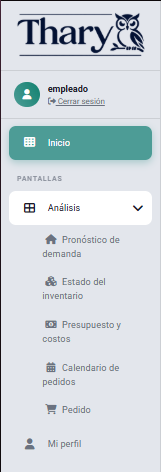
\includegraphics[height=0.25\textheight]{templatefigures/ux_sidebar_empleado.png}
        \caption{Sidebar de empleado}
        \label{fig:ux_sidebar_empleado}
    \end{subfigure}
    \hspace{1cm}
    \begin{subfigure}[b]{0.42\textwidth}
        \centering
        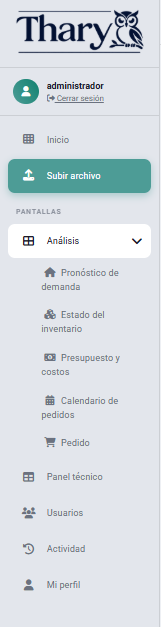
\includegraphics[height=0.25\textheight]{templatefigures/ux_sidebar_administrador.png}
        \caption{Sidebar de administrador}
        \label{fig:ux_sidebar_administrador}
    \end{subfigure}
\end{figure}

\begin{figure}[H]
    \centering
    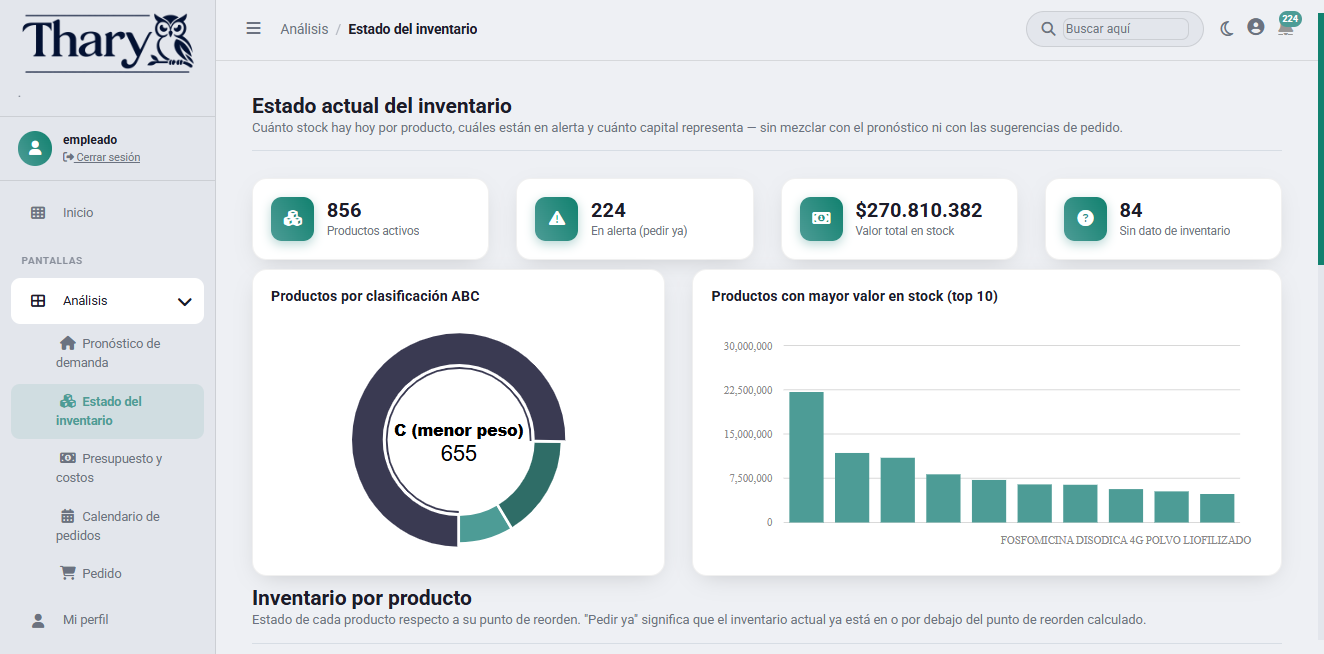
\includegraphics[height=0.25\textheight]{templatefigures/ux_estado_inventario.png}
    \caption{Estado del inventario}
    \label{fig:ux_estado_inventario}
\end{figure}

\begin{figure}[H]
    \centering
    \begin{subfigure}[b]{0.85\textwidth}
        \centering
        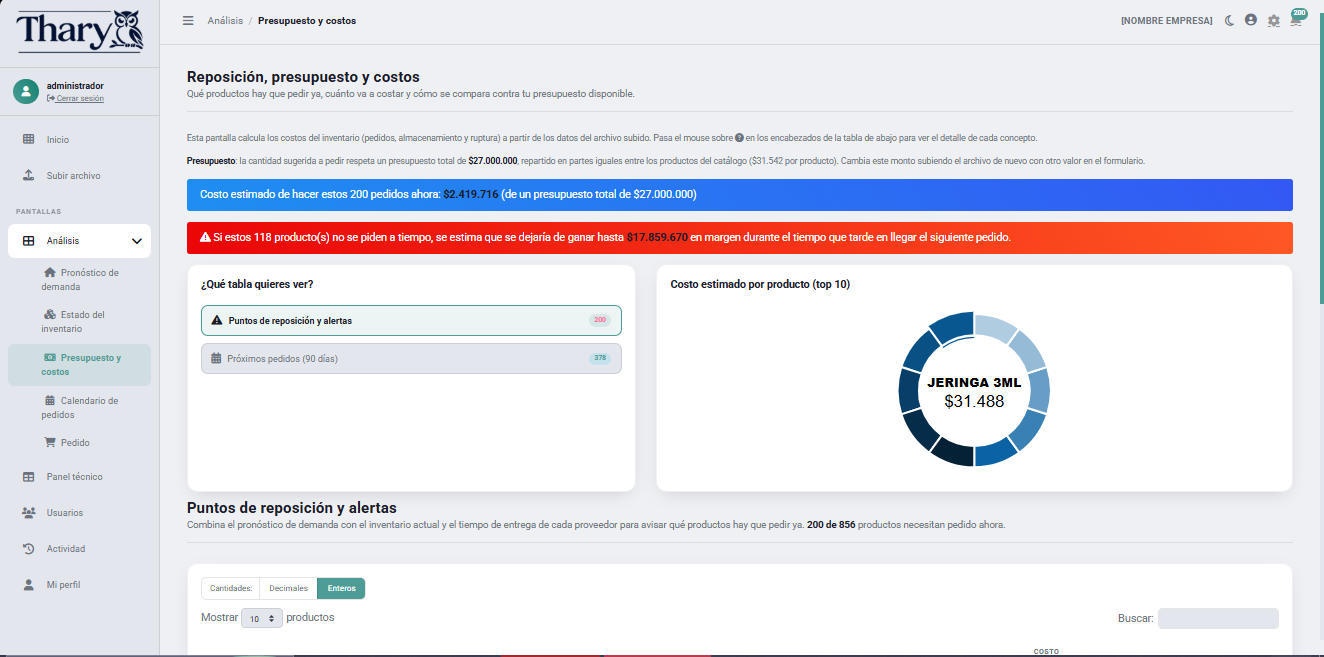
\includegraphics[width=\textwidth]{templatefigures/ux_presupuesto.png}
        \caption{Presupuesto}
        \label{fig:ux_presupuesto}
    \end{subfigure}

    \vspace{0.4cm}

    \begin{subfigure}[b]{0.85\textwidth}
        \centering
        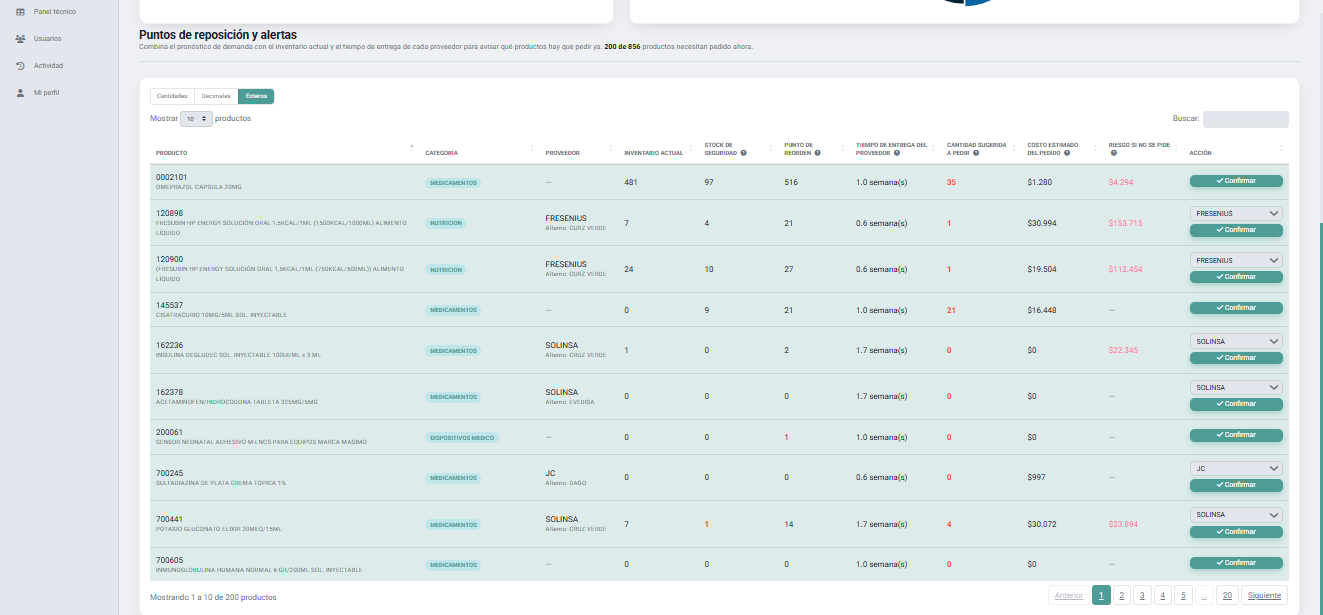
\includegraphics[width=\textwidth]{templatefigures/ux_reposicion_alertas.png}
        \caption{Alertas de reposición}
        \label{fig:ux_reposicion_alertas}
    \end{subfigure}
\end{figure}

La gestión de pedidos se puede ver en tres vistas: los pedidos sugeridos pendientes de confirmar, el historial de pedidos ya confirmados, y los próximos pedidos estimados según el calendario de reposición.

\begin{figure}[H]
    \centering
    \begin{subfigure}[b]{0.85\textwidth}
        \centering
        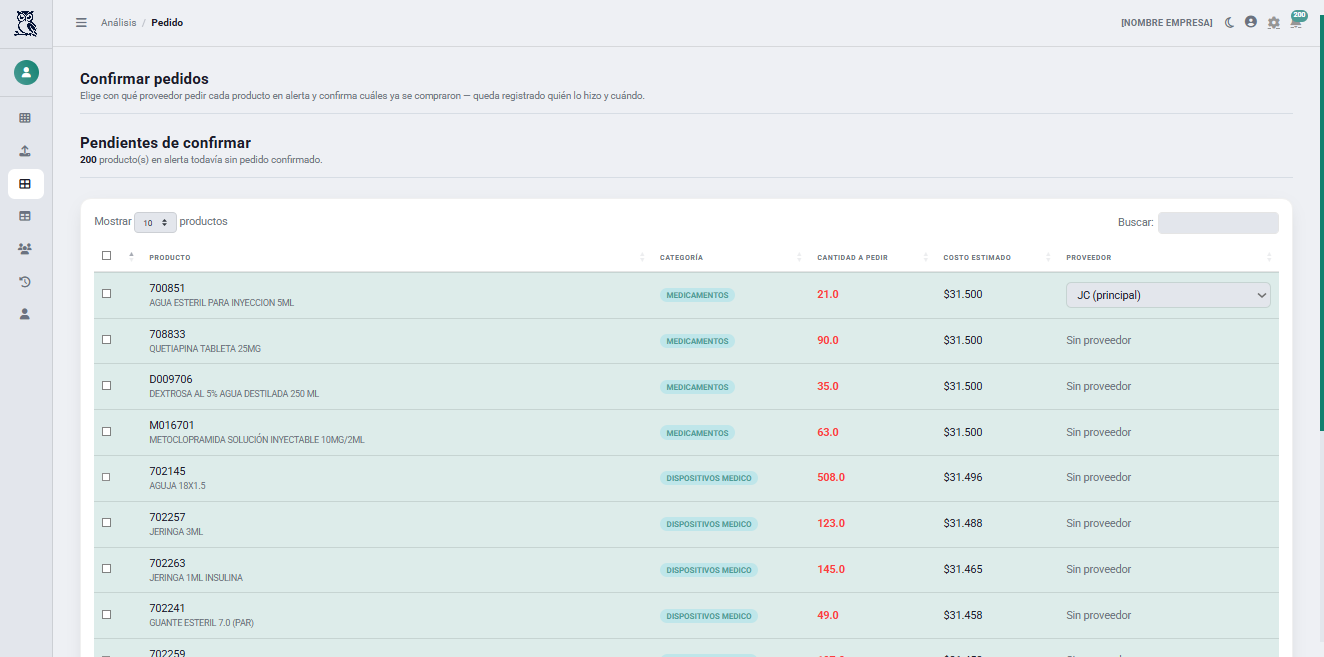
\includegraphics[width=\textwidth]{templatefigures/ux_pedidos.png}
        \caption{Lista de Pedidos}
        \label{fig:ux_pedidos}
    \end{subfigure}

    \vspace{0.4cm}

    \begin{subfigure}[b]{0.85\textwidth}
        \centering
        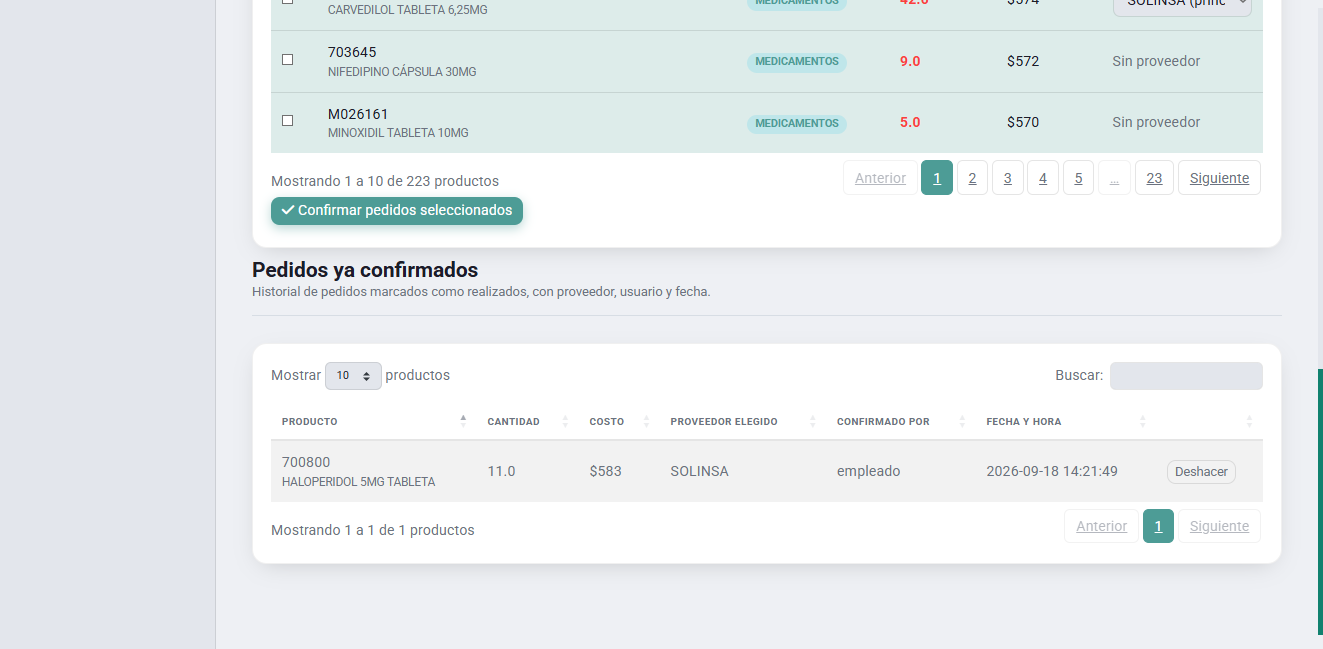
\includegraphics[width=\textwidth]{templatefigures/ux_pedidos_confirmados.png}
        \caption{Pedidos confirmados}
        \label{fig:ux_pedidos_confirmados}
    \end{subfigure}
\end{figure}

\begin{figure}[H]
    \centering
    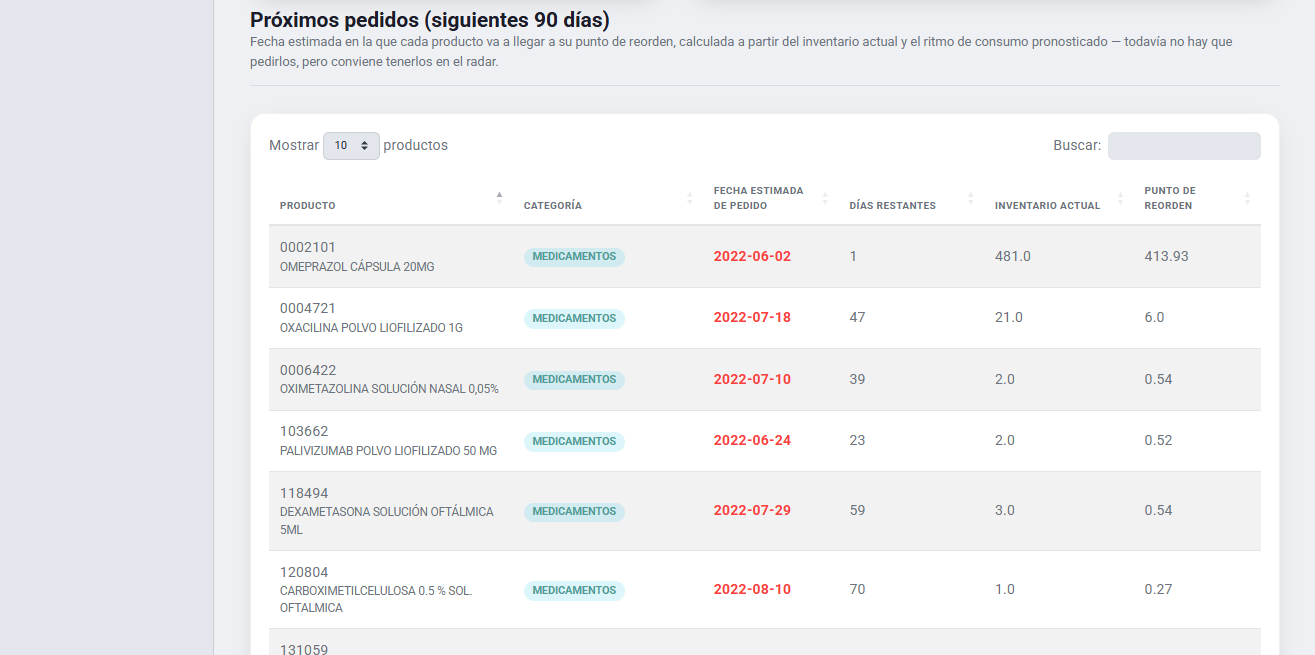
\includegraphics[height=0.25\textheight]{templatefigures/ux_prox_pedidos.png}
    \caption{Próximos pedidos}
    \label{fig:ux_prox_pedidos}
\end{figure}

\begin{figure}[H]
    \centering
    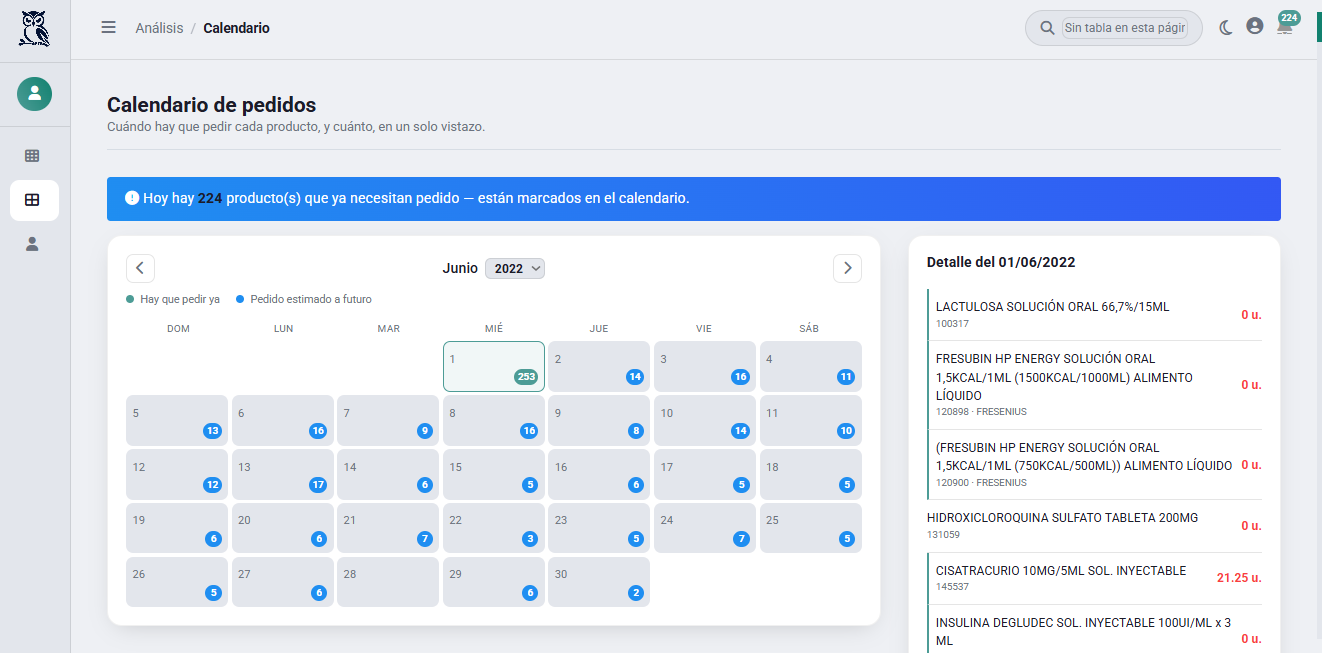
\includegraphics[height=0.25\textheight]{templatefigures/ux_calendario_pedidos.png}
    \caption{Calendario de pedidos}
    \label{fig:ux_calendario_pedidos}
\end{figure}

Una vez finalizadas sus tareas, los usuarios pueden cerrar sesión en su cuenta.

\begin{figure}[H]
    \centering
    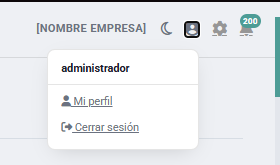
\includegraphics[width=0.5\textwidth]{templatefigures/ux_cerrar_sesion.png}
    \caption{Cerrar sesión}
    \label{fig:ux_cerrar_sesion}
\end{figure}

Los criterios de usabilidad que fueron tomados en cuenta fueron:

\begin{itemize}
    \item Uso de alertas visuales codificadas por color para indicar fácilmente que productos se encuentran en o por debajo de su punto de reposición y requieren ser reabastecidos inmediatamente.
    
    \begin{figure}[H]
    \centering
    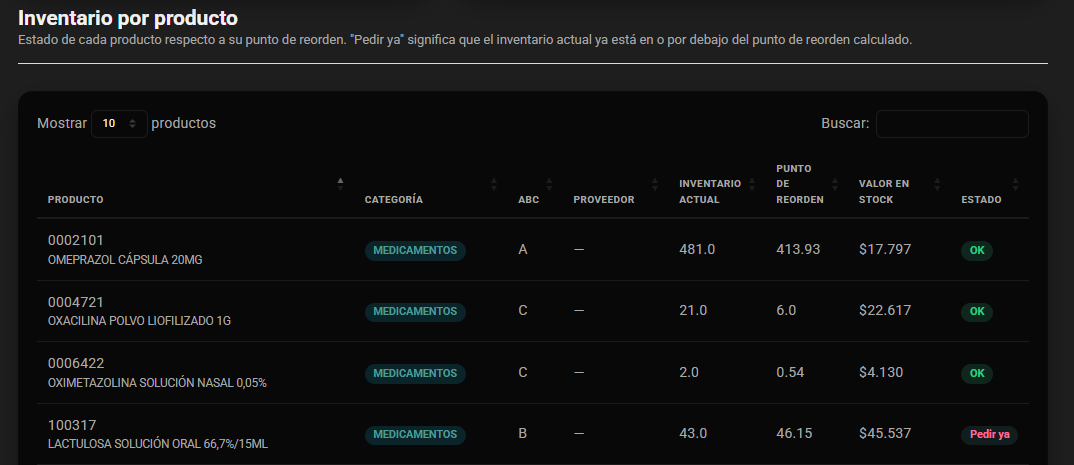
\includegraphics[width=0.5\textwidth]{templatefigures/ux_alertas_visuales.png}
    \caption{Alertas visuales}
    \label{fig:ux_alertas_visuales}
    \end{figure}

    \item Cuando un usuario con el rol de empleado inicie sesión, pero su respectivo administrador no subió ningún archivo csv, en vez de ver la pantalla del dashboard, verá una pantalla con el mensaje de que una vez el admin cargue el archivo, podrá ver los análisis.

    \begin{figure}[H]
    \centering
    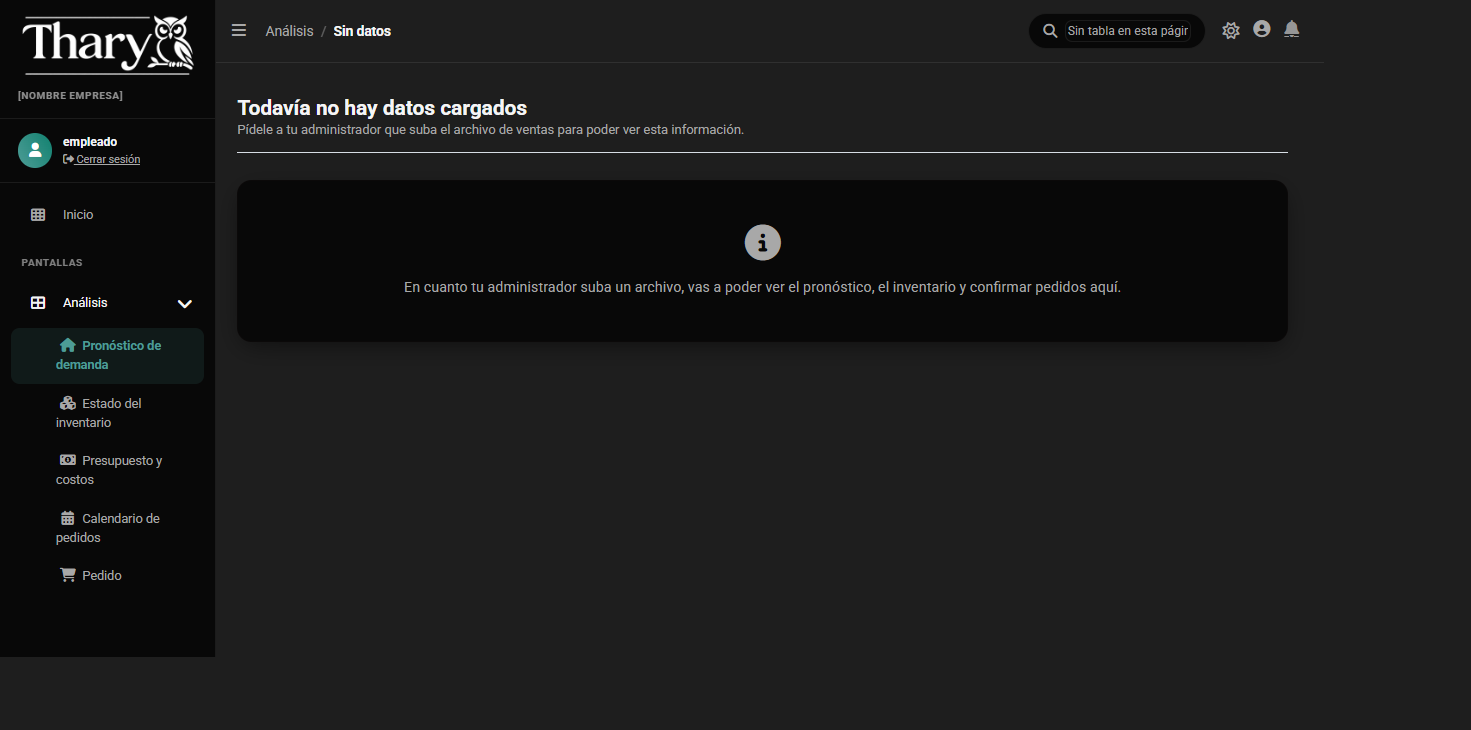
\includegraphics[width=0.5\textwidth]{templatefigures/ux_dashboard_empleado.png}
    \caption{Dashboard del empleado}
    \label{fig:ux_dashboard_empleado}
    \end{figure}
    
    \item El sistema cuenta con un modo oscuro y modo claro para que el usuario pueda escoger según sus preferencias, mejorando la usabilidad ofreciendo ventajas como comodidad visual, menor fatiga en uso prolongado, contraste, etc.

    \begin{figure}[H]
    \centering
    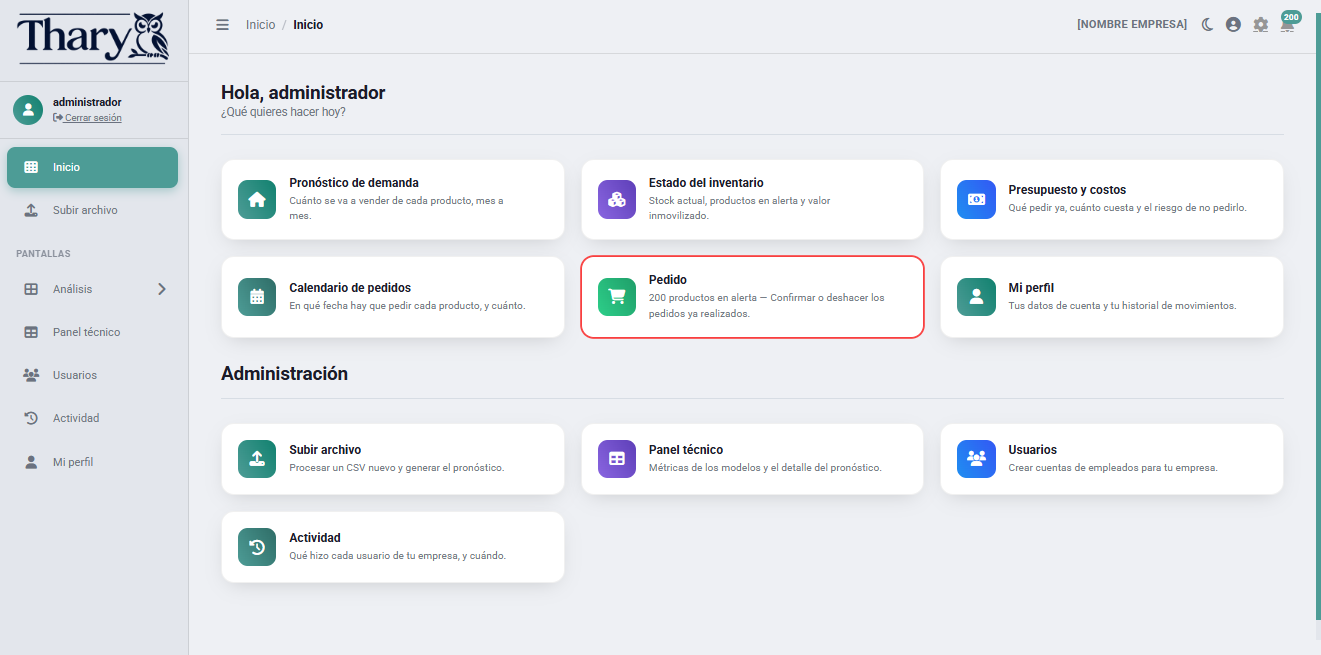
\includegraphics[width=0.5\textwidth]{templatefigures/ux_dashboard_claro.png}
    \caption{Dashboard en modo claro}
    \label{fig:ux_dashboard_claro}
    \end{figure}

    \item Thary cuenta con una versión mobile, la cual le permite al usuario poder acceder a todas las funcionalidades de la versión de escritorio desde su teléfono móvil.

        \begin{figure}[H]
    \centering
    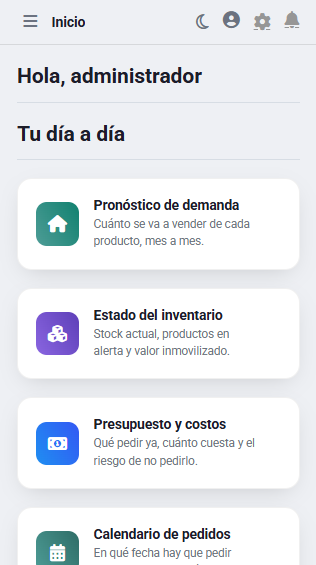
\includegraphics[width=0.5\textwidth]{templatefigures/ux_dashboard_mobile.png}
    \caption{Dashboard en modo mobile}
    \label{fig:ux_dashboard_mobile}
    \end{figure}
\end{itemize}

En cuanto a criterios de accesibilidad, se tomaron en cuenta los criterios de usabilidad, pero no se tomaron en cuenta mecanismos adicionales para hacer más accesible el sistema como algún tipo de lector de pantalla para personas con discapacidad visual, o implementar un sistema de navegación completa por teclado para alguna persona que no pueda usar un mouse. Estas falencias se reconocen como una limitación del diseño actual, y se espera mejorarlas en el futuro. 
